\documentclass[mathserif,slidestop,compress,red]{beamer}
%\usepackage[utf8]{inputenc}
\usepackage{graphicx}
\usepackage{caption}
\usepackage{listings}

\usetheme{Antibes}

\usepackage{fontspec}
\usepackage{xltxtra}
\setmonofont{Courier 10 Pitch}
\setromanfont{LMMathItalic7 Bold}
\setsansfont{Ubuntu}

\beamertemplatenavigationsymbolsempty

\title{Control-Flow Integrity Checking}
\subtitle{Vortrag im Hauptseminar Betriebssysteme}
\author{Hermann Loose}
\date{03.02.2012}

\definecolor{light-gray}{gray}{0.7}

\DeclareCaptionFont{white}{\color{white}}
\DeclareCaptionFormat{listing}{\colorbox{gray}{\parbox{\textwidth}{\hspace{0.9em}#1#2#3}}}
\captionsetup[lstlisting]{format=listing,labelfont=white,textfont=white,font={sf}}

\AtBeginSection[] {
  \begin{frame}[plain]
    \tableofcontents[currentsection]
  \end{frame}
  \addtocounter{framenumber}{-1}
}

\begin{document}

\definecolor{keywords}{RGB}{255,0,90}
\definecolor{comments}{RGB}{100,100,100}
\lstset{
  language=[x86masm]Assembler,
  basicstyle=\ttfamily
  %frame=lines
}

\frame[plain]{\titlepage}

\begin{frame}
  \frametitle{Kurz etwas zur Benennung …}
  bevor später Verwirrung aufkommt:
  \begin{itemize}
    \item \textbf{Control-Flow Integrity Checking} \\ ist eine generelle Idee % und der Titel
    \item \textbf{Control-Flow Integrity} \\ ist ein Verfahren % das betrachtete Microsoft'sche Verfahren dazu
    \item \textbf{Software Signatures} \\ ist ein anderes Verfahren
  \end{itemize}
  \begin{flushright}
    Ja, etwas unglücklich.
  \end{flushright}
\end{frame}

\part{1}
\section{Control-Flow Integrity}

\subsection{Motivation}

\begin{frame}[fragile]
  \frametitle{Das Problem}
  \begin{lstlisting}
  void foo(void) {
    char buf[30];
    gets(buf);
    printf("%s\n", buf);
  }
  \end{lstlisting}
\end{frame}

\begin{frame}
  \frametitle{Das Problem}
  \begin{itemize}
    \item dynamischer Kontrollfluss
    \begin{itemize}
      \item Funktionspointer
      \item Returns
    \end{itemize}
    \item Vertrauen auf Integrität des Datensegments
    \begin{itemize}
      \pause
      \item also am besten abschaffen!
    \end{itemize}
  \end{itemize}
\end{frame}

\begin{frame}
  \frametitle{Angreifermodell}
  Der Angreifer hat
  \begin{itemize}
    \item volle Kontrolle über Datensegment
  \end{itemize}
  \pause
  das heißt wir rechnen mit
  \begin{itemize}
    \item klassischen, Stack-basierten Pufferüberläufen
    \item Heap-basierten Pufferüberläufen
  \end{itemize}
  \pause
  wollen aber Folgendes \textbf{verhindern}:
  \begin{itemize}
    \item \emph{jump-to-libc} Angriffe
    \item Return-Oriented Programming
    \item \emph{pointer subterfuge} Angriffe
  \end{itemize}
  \vspace{0.5em}
  Für ein vereinfachtes Maschinenmodell existiert in [2] ein formaler Beweis.
\end{frame}

\subsection{Konzept}

\begin{frame}
  \frametitle{Control-Flow Graph (CFG)}
  \begin{itemize}
    \item Knoten sind Codeabschnitte (\emph{basic blocks}) mit linearem Kontrollfluss
    % TODO(hermannloose): Lassen wir hier eigentlich direkte Sprünge schon weg?
    \item Kanten zeigen möglichen Kontrollfluss zwischen Knoten an, hauptsächlich z.B. Funktionsaufrufe und Returns
    \item Weg im CFG = erlaubte Ausführungsreihenfolge
    \item muss im Vorhinein feststehen
    \begin{itemize}
      \item Analyse von Quellcode
      \item Analyse von Binaries
      \item Profiling der Ausführung
      \item als Ausdruck einer vorgegebenen Security Policy
    \end{itemize}
    \item \textbf{hier:} statische Analyse von Binaries
  \end{itemize}
\end{frame}

\begin{frame}
  \frametitle{Annahmen}
  \begin{itemize}
    \item[NWC] Non-Writable Code Memory
    \begin{itemize}
      \item auf den meisten Systemen gegeben
      \pause
      \item und kann später von CFI selbst erledigt werden
    \end{itemize}
    \pause
    \item[NXD] Non-Executable Data Memory
    \begin{itemize}
      \item in Hardware auf x86
      \item in Software möglich\footnote<3->{PaX — http://pax.grsecurity.net}
      \pause
      \item und kann später von CFI selbst erledigt werden
    \end{itemize}
  \end{itemize}
\end{frame}

\begin{frame}
  \frametitle{Instrumentierung}
  \begin{itemize}
    \item entsprechend dem CFG,
    \item für alle Kontrollflusstransfers mit berechnetem Ziel,
    \item und alle erlaubten Ziele.
    \pause
    \vspace{1em}
    \item vor jedem Ziel die ID seiner Äquivalenzklasse,\\ als Daten
    oder Operand einer „\texttt{label}“-Instruktion
    \item vor jeder Quelle ein ID-Vergleich der Äquivalenzklasse des
    Ziels zur Laufzeit mit der erlaubten
  \end{itemize}
\end{frame}

\subsection{Implementierung}

\begin{frame}[fragile]
  \frametitle{Ausgangspunkt}
  \begin{lstlisting}[title=Quelle]



  jmp ecx              ; jump to dst
  \end{lstlisting}
  \begin{lstlisting}[title=Ziel]

  mov eax, [esp+4]     ; dst
  \end{lstlisting}
\end{frame}

\begin{frame}[fragile]
  \frametitle{Instrumentierung — Variante 1}
  \begin{lstlisting}[title=Quelle]
  cmp [ecx], 12345678h ; comp ID & dst
  jne error_label      ; if != fail
  lea ecx, [ecx+4]     ; skip ID at dst
  jmp ecx              ; jump to dst
  \end{lstlisting}
  \begin{lstlisting}[title=Ziel]
  ; data 12345678h     ; ID
  mov eax, [esp+4]     ; dst
  \end{lstlisting}
  \pause
  \begin{flushright}
    Was ist hier schlecht?
  \end{flushright}
\end{frame}

%\begin{frame}[fragile]
%  \frametitle{Quelle — erster Versuch}
%  \begin{lstlisting}
%  cmp [ecx], 12345678h ; 81 39 78 56 34 12
%  jne error_label      ; 75 13
%  lea ecx, [ecx+4]     ; 8D 49 04
%  jmp ecx              ; FF E1
%  \end{lstlisting}
%\end{frame}

\begin{frame}[fragile]
  \frametitle{Instrumentierung — Variante 1}
  \begin{lstlisting}[title=Quelle,escapechar=!]
  cmp [ecx], !\colorbox{light-gray}{12345678h}! ; 81 39 !\emph{\colorbox{light-gray}{78 56 34 12}}!
  jne error_label      ; 75 13
  lea ecx, [ecx+4]     ; 8D 49 04
  jmp ecx              ; FF E1
  \end{lstlisting}
  \textbf{Problem:} die ID ist in die \texttt{cmp} Instruktion eingebettet, \\ macht
  damit \texttt{jne error\_label} zu einem gültigen Ziel
\end{frame}

\begin{frame}
  \frametitle{Annahmen, ergänzt}
  \begin{itemize}
    \item[NWC] Non-Writable Code Memory
    \begin{itemize}
      \item auf den meisten Systemen gegeben
    \end{itemize}
    \item[NXD] Non-Executable Data Memory
    \begin{itemize}
      \item in Hardware auf x86
      \item in Software möglich
    \end{itemize}
    \begin{flushleft}
      \textbf{und außerdem}
    \end{flushleft}
    \item[UNQ] Unique IDs
    \begin{itemize}
      \item IDs ausschließlich vor möglichen Zielen
      \item mindestens 32 Bit groß, gegen Angreifer mit Glück, Wissen oder Ausdauer
    \end{itemize}
  \end{itemize}
\end{frame}

\begin{frame}[fragile]
  \frametitle{Instrumentierung — Variante 2}
  \begin{lstlisting}[title=Quelle]
  mov eax, 12345677h ; load ID-1
  inc eax            ; increment ID
  cmp [ecx-4], eax   ; compare w/ dst
  jne error_label    ; if != fail
  jmp ecx            ; jump to label
  \end{lstlisting}
  \begin{lstlisting}[title=Ziel]
  prefetchnta        ; label
     [12345678h]     ;    ID
  mov eax, [esp+4]   ; dst
  \end{lstlisting}
\end{frame}

\begin{frame}
  \frametitle{Beobachtungen}
  \begin{itemize}
    \item gröberer CFG durch Annahme von Ziel-Äquivalenzklassen
    \begin{itemize}
      \item ignoriert z.B. virtuelle Methoden
    \end{itemize}
    \item Returns nicht auf jüngsten Aufrufort beschränkt
    \pause
    \vspace{1em}
    \item vermeidbar durch Codeduplizierung
    \begin{itemize}
      \item Äquivalenzannahme herstellbar
      \item Extremfall: komplettes Inlining
    \end{itemize}
    \item Verfeinerung der Instrumentierung denkbar
    \pause
    \vspace{1em}
    \item allerdings gibt bereits ein grober CFG einige Garantien
    \begin{itemize}
      \item keine Sprünge in die Mitte von Funktionen
      \item nur Returns an Aufruforte, etc.
    \end{itemize}
  \end{itemize}
\end{frame}

\subsection{CFI als Basis für andere Mechanismen}

\begin{frame}
  \frametitle{CFI als Basis für andere Mechanismen}
  \begin{itemize}
    \item [IRM] Inlined Reference Monitors
    \begin{itemize}
      \item erleichtert durch die Garantien von CFI
      \item keine Umgehung möglich
    \end{itemize}
    \item [SFI] Software Fault Isolation
    \begin{itemize}
      \item reduzierter Overhead z.B. in Schleifen
      \item nicht jeder Speicherzugriff muss überprüft werden
    \end{itemize}
  \end{itemize}
\end{frame}

\lstset{language=C}

\begin{frame}[fragile]
  \frametitle{CFI für schnellere SFI}
  \begin{lstlisting}[escapechar=!]
  int compute_sum(int a[], int len)
  {
    int sum = 0;
    for (int i = 0; i < len; ++i) {
      !\colorbox{light-gray}{sum += a[i];}!
    }
    return sum;
  }
  \end{lstlisting}
  \vspace{1em}
  \begin{itemize}
    \item Speicherzugriff \textbf{\texttt{a[i]}} soll jeweils geprüft werden
  \end{itemize}
\end{frame}

\lstset{language=[x86masm]Assembler}

\begin{frame}[fragile]
  \frametitle{CFI für schnellere SFI}
  \begin{lstlisting}
        ...
        mov ecx, 0h          ; int i = 0
        mov esi, [esp+8]     ; a[] base ptr
        and esi, 20FFFFFFh   ; SFI masking
  LOOP: add eax, [esi+ecx*4] ; sum += a[i]
        inc ecx              ; ++i
        cmp ecx, edx         ; if i < len
        jl  LOOP             ; repeat
  \end{lstlisting}
  \vspace{1em}
  \begin{itemize}
    \item CFI garantiert korrekten Kontrollfluss, \textbf{\texttt{esi}} und \textbf{\texttt{ecx}} enthalten also nie unerwartete Werte
    \item ein einzelner Check genügt
  \end{itemize}
\end{frame}

% TODO(hermannloose): Messwerte hierzu anführen?
% TODO(hermannloose): Ist dazu je das angekündigte Follow-Up erschienen?

\begin{frame}
  \frametitle{Software Memory Access Control (SMAC)}
  \begin{itemize}
    \item flexible Beschränkungen von Speicherzugriffen
    \begin{itemize}
      \item bestimmte Speicherregionen nur von bestimmten Funktionen aus erreichbar (z.B. aus IRMs)
      \item in Codebereiche darf nicht geschrieben werden (NWC)
      \item in Datenbereiche darf nicht gesprungen werden (NXD)

    \end{itemize}
  \end{itemize}
\end{frame}

\begin{frame}[fragile]
  \frametitle{Software Memory Access Control}
  \begin{lstlisting}[title={Call, mit SMAC}]
  and  eax, 40FFFFFFh ; mask func ptr
  cmp  [eax-4], ID    ; compare dst w/ ID
  jne error_label     ; if != fail
  call eax            ; call func ptr
  prefetchnta ID      ; label ID, for ret
  ...
  \end{lstlisting}
\end{frame}

\begin{frame}[fragile]
  \frametitle{Software Memory Access Control}
  \begin{lstlisting}[title={Return, mit SMAC}]
  mov  ecx, [esp]     ; load return dst
  and  ecx, 40FFFFFFh ; mask return dst
  cmp  [ecx-4], ID    ; comp dst w/ ID
  jne  error_label    ; if != fail
  add  esp, 4h        ; pop 4
  jmp  ecx            ; jump return dst
  \end{lstlisting}
\end{frame}

% TODO(hermannloose): Drin lassen? Wird lang.
\subsection{Messungen}

\begin{frame}
  \frametitle{Messungen}
  \begin{itemize}
    \item SPEC Benchmarks in Windows XP SP2 Safe Mode
    \item Pentium 4 x86 mit 1.8GHz und 512MB RAM\footnote{veröffentlicht 2005}
    \item Instrumentierung etc. etwa 10 Sekunden
    \item Overhead: etwa 8\% in der Größe, etwa 16\% in der Zeit
    \vspace{1em}
    \item zumindest ein Experiment zur Sicherheit; 18 Buffer Overflow Exploits aus [4], alle vereitelt
    \item ansonsten aber eher unspezifisch und theoretisch
  \end{itemize}
\end{frame}

\part{2}
\section{Software Signatures}

\subsection{Motivation}

\begin{frame}
  \frametitle{Software Signatures}
  \textbf{Fokus:} Erkennung von transienten Hardwarefehlern\footnote{http://en.wikipedia.org/wiki/ARGOS\_(satellite)}
  \begin{itemize}
    \pause
    \item CFG bleibt prinzipiell gleich
    \pause
    \item jeder Knoten erhält eine Signatur
    \pause
    \item ein Register hält die Laufzeitsignatur
    \pause
    \item Laufzeitsignatur beim Eintritt in den Knoten geprüft
    \pause
    \item Kontrollflusstransfers modifizieren die Laufzeitsignatur
    \pause
    \item unerwartete (oder fehlende) Transfers lassen die Laufzeitsignatur ungültig werden
  \end{itemize}
\end{frame}

\subsection{Konzept}

\begin{frame}
  \frametitle{Vorgehen}
  \begin{itemize}
    \item jeder Knoten $v_i$ hat eine eindeutige Signatur $s_i$
    \pause
    \item \emph{Global Signature Register} (GSR) hält die Laufzeitsignatur~$G$
    \pause
    \item im Knoten $v_i$ sollte $G = s_i$ gelten, \\
          sonst ist ein Fehler aufgetreten
    \pause
    \item im Knoten $v_i$ heißt $G$ auch $G_i$
  \end{itemize}
\end{frame}

\begin{frame}
  \frametitle{Erlaubter Transfer von $v_s$ zu $v_d$}
  \begin{itemize}
    \pause
    \item Signaturfunktion $f$
    \item in $v_d$ bestimmt $f$ ein neues $G$
    \pause
    \item aus $G_s$ muss ein passendes $G_d = s_d$ werden
    \pause
    \item in $v_d$ wird $d_d = s_s \oplus s_d$ gespeichert
    \pause
    \item als neue Laufzeitsignatur wird berechnet
    \begin{align*}
    G_d = f(G_s, d_d) &= s_s \oplus d_d \\
    &= s_s \oplus ( s_s \oplus s_d ) \\
    &= s_d
    \end{align*}
  \end{itemize}
\end{frame}

\begin{frame}
  \frametitle{Unerlaubter Transfer von $v_e$ zu $v_d$}
  \begin{itemize}
    \pause
    \item in $v_e$ enthält das GSR $G_e = s_e$
    \pause
    \item in $v_d$ steht $d_d = s_s \oplus s_d$ \\
          (für erlaubten Transfer von $v_s$ nach $v_d$)
    \pause
    \item als neue Laufzeitsignatur wird berechnet
    \begin{align*}
    G_d = f(G_e, d_d) &= s_e \oplus d_d \\
    &= s_e \oplus ( s_s \oplus s_d ) \\
    &\neq s_d
    \end{align*}
  \end{itemize}
\end{frame}

\begin{frame}
  \frametitle{Unerlaubter Transfer in die Mitte eines Knotens}
  \begin{itemize}
    \pause
    \item in $v_1$ enthält das GSR $G_1 = s_1$
    \pause
    \item unerlaubter Transfer in die Mitte von $v_2$
    \pause
    \item Check und Update von $G$ werden übersprungen
    \pause
    \item erlaubter Transfer von $v_2$ nach $v_3$
    \item \textbf{aber:} GSR enthält weiterhin $s_1$
    \pause
    \item in $v_3$ steht $d_3 = s_2 \oplus s_3$ \\
          (für erlaubten Transfer von $v_2$ nach $v_3$)
    \pause
    \item als neue Laufzeitsignatur wird berechnet
    \begin{align*}
    G_3 = f(G_1, d_3) &= s_1 \oplus d_3 \\
    &= s_1 \oplus ( s_2 \oplus s_3 ) \\
    &\neq s_3
    \end{align*}
  \end{itemize}
\end{frame}

\begin{frame}
  \frametitle{Mehrere Eingangskanten}
  \begin{itemize}
    \item zwei Knoten $v_1$ und $v_2$ mit erlaubten Transfers zu $v_3$
    \item $v_3$ ist ein sogenannter \emph{Branch Fan-In} Knoten
    \item in $v_3$ steht z.B. $d_3 = s_1 \oplus s_3$
    \item was passiert mit Transfers von $v_2$?
    \vspace{1em}
    \pause
    \item möglich wäre $s_1 = s_2$ zu setzen
    \pause
    \item und alle Ziele von $v_1$ und $v_2$ würden äquivalent
  \end{itemize}
\end{frame}

\begin{frame}
  \frametitle{Mehrere Eingangskanten}
  stattdessen:
  \begin{itemize}
    \item ein weitere (Laufzeit–) Signatur $D$
    \pause
    \item in $v_1$ wird $D$ genullt
    \pause
    \item in $v_2$ wird $D$ auf $s_1 \oplus s_2$ gesetzt
    \pause
    \item in $v_3$ wird $G_3$ berechnet:
    \begin{columns}
      \begin{column}{0.5\textwidth}
      \begin{align*}
      G_3 &= f(G_1, d_3) \oplus D \\
      &= s_1 \oplus d_3 \\
      &= s_1 \oplus s_1 \oplus s_3 \\
      &= s_3
      \end{align*}
      \end{column}

      \begin{column}{0.5\textwidth}
      \begin{align*}
      G_3 &= f(G_2, d_3) \oplus D \\
      &= s_2 \oplus d_3 \oplus s_1 \oplus s_2 \\
      &= s_1 \oplus s_1 \oplus s_3 \\
      &= s_3
      \end{align*}
      \end{column}
    \end{columns}
  \end{itemize}
\end{frame}

\begin{frame}
  \frametitle{Aliasing-Problem}
  \begin{itemize}
    \item mehrere Knoten teilen sich mehrere Branch Fan-In Knoten als Ziele (aber nicht alle)
  \end{itemize}
  \begin{center}
  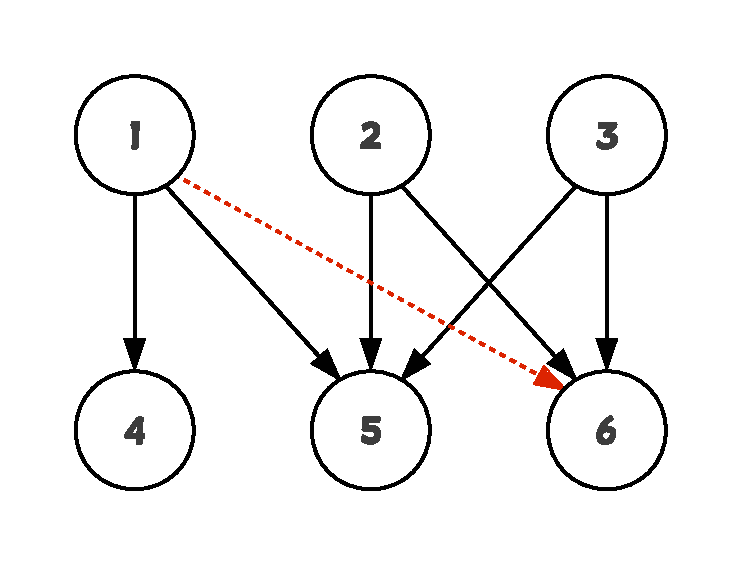
\includegraphics[width=0.7\textwidth]{aliasing}
  \end{center}
\end{frame}

\begin{frame}
  \frametitle{Aliasing-Problem}
  \begin{itemize}
    \item mehrere Knoten teilen sich mehrere Branch Fan-In Knoten als Ziele (aber nicht alle)
    \item tritt auf wenn $d_i = s_s \oplus s_i, d_j = s_s \oplus s_j$ gilt, aber die Mengen der
    Vorgänger von $v_i$ und $v_j$ nicht gleich sind
    \begin{itemize}
      \item ein unerlaubter Transfer von $v_1$ zu $v_6$ würde im Beispiel nicht erkannt
    \end{itemize}
    \pause
    \item nur bei Transfer zur ersten Instruktion im Knoten
    \item kann über Hamming-Distanz zwischen Startadressen von Knoten zum Teil gelöst werden
  \end{itemize}
\end{frame}

\subsection{Messungen}

\begin{frame}
  \frametitle{Messungen}
  \begin{itemize}
    \item sieben Benchmarks mit zufällig eingefügten Fehlern
    \begin{itemize}
      \item Ersetzung von Sprüngen durch NOPs
      \item Einfügung von unbedingten Sprüngen
      \item Veränderung von Sprungoperanden
    \end{itemize}
    \item durchgeführt auf SGI Indigo (R4400 MIPS)\footnote{veröffentlicht 2000}
    \item durch OS festgestellte Abstürze werden nicht betrachtet
    \item ohne Signaturen: 33,7\% unentdeckt falsche Ergebnisse
    \item mit Signaturen: 3,1\% unentdeckt falsche Ergebnisse
    \item Overhead: 45,2\% in der Größe, 43,1\% in der Zeit
    \begin{itemize}
      \item häufig sehr kleine Blöcke (ca. 7 Instruktionen)
      \item kann reduziert werden, wenn Signaturen sporadischer überprüft werden
    \end{itemize}
  \end{itemize}
\end{frame}

\section*{}

\begin{frame}
  \frametitle{Quellen}
  \begin{enumerate}
    \item \emph{Control-Flow Integrity} \\ M. Abadi, M. Budiu, Ú. Erlingsson, J. Ligatti — 2005
    \item \emph{A Theory of Secure Control Flow} \\ M. Abadi, M. Budiu, Ú. Erlingsson, J. Ligatti — 2005
    \item \emph{Control-Flow Checking by Software Signatures} \\ N. Oh, P. Shirvani, E. McCluskey — 2000
    \item \emph{A Comparison of Publicly Available Tools for \\ Dynamic Buffer Overflow Prevention} \\
        J. Wilander, M. Kamkar — 2003
  \end{enumerate}
\end{frame}

{
\setbeamercolor{normal text}{bg=black}
\setbeamercolor{whitetext}{fg=white}
\begin{frame}[c,plain]
  \begin{center}
    \usebeamercolor[fg]{whitetext}
    Vielen Dank für die Aufmerksamkeit!
  \end{center}
\end{frame}
}

\end{document}
